\chapter{DUST Postprocessor}
\label{ch:Post}

The DUST postprocessor is used to generate meaningful data from the binary 
results generated during the execution of the solver. While as discussed in 
\ref{sec:OutputFilesFormat} it is possible to look at the content of the hdf5 
results, these being based on the singularities intensities on the surface provide 
little insight on the solution of the solver. 

The postprocessor takes the specified results and use them to obtain a variety of 
different processed data, from visualizations to loads. 

The preprocessor is executed simply invoking the executable \texttt{dust\_post} 
in the desired folder. The input file containing all the required informations 
for the execution of the postprocessor must be passed as argument to the command call. 
If not provided explicitly the preprocessor automatically tries to read the default 
input file \texttt{dust\_post.in}.
\begin{command}[caption={Postprocessor command looking for input file 
  \texttt{input\_file\_name.in}}]
  dust_post input_file_name.in
\end{command}

\begin{command}[caption={Postprocessor command looking for 
default input file \texttt{dust\_post.in}}, label={command:dust_post_default}]
  dust_post
\end{command}

The different possible analysis that can be performed on the results are:
\begin{itemize}
\item \textbf{Integral loads}: history of loads acting on the geometry or parts 
      of the geometry
\item \textbf{Visualizations}: visualization of the surface solution 
      on the geometry and of the wake
\item \textbf{Probes}: Time history of certain variables probed in a 
      set of specified points
\item \textbf{Flow fields}: Visualization of the flow field in a structured 
      block domain
\item \textbf{Sectional loads}: distribution of the loads along a direction 
      on long aspect ratio components (i.e. wings or blades)
\end{itemize}


\section{input file}
\label{sec:Post_InputFile}

The input file of the postprocessor contains first all the information 
required for retrieving the correct results and to process the data 
(model parameters etc.) and then in separate sections all the analyses 
that are requested. An arbitrary number of analyses can be requested in 
a single input file, however it is also possible to group the analyses 
in different input files then invoked multiple times as different inputs 
for the postprocessor. 

The format is the same as all the other input files, as already specified 
in section\ref{sec:InputFilesFormat}.

A generic input file describing the main input is:

\begin{inputfile}[frame=single, caption={dust\_post.in}, label={file:dust_post.in}]
!--- Data Names ---
data_basename = ./Output/sim_results
basename =     ./Postpro/postpro_output

!--- Model Parameters (as in solver) ---
far_field_ratio_doublet = 10.0
far_field_ratio_source = 10.0
doublet_threshold = 1.0e-6
rankine_rad = 0.1
vortex_rad = 0.1
cutoff_rad = 0.001

analysis = {

type = viz  
name = vis01
start_res = 1
end_res   = 100 
step_res  = 1
format = vtk
wake = T
variable = vorticity 
}

analysis = {

type = integral_loads
name = load01
start_res = 1
end_res   = 100 
step_res  = 1
format = dat
average = F
component = all
reference_tag = RotorHub
}

\end{inputfile}

\begin{itemize}
\item \param{data\_basename}: \textit{required:} yes. \textit{multiple:} no. 

Base name (with path) of the data which must be analysed.

\item \param{basename}: \textit{required:} yes. \textit{multiple:} no. 

Base name (with path) of the postprocessing results

\item \param{far_field_ratio_doublet}: \textit{required:} no. 
\textit{multiple:} no. \textit{default:} 10

Ratio with respect to element length to set the thresholds for far field approximation. 
Same as in solver input file \ref{file:dust.in}.

\item \param{far_field_ratio_source}: \textit{required:} no. \textit{multiple:} no. 
\textit{default:} 10

As for \param{far_field_ratio_doublet} determines the threshold after which 
far field approximations are employed, just for sources. Same as in solver 
input file \ref{file:dust.in}.

\item \param{doublet_threshold}: \textit{required:} no. \textit{multiple:} no. 
\textit{default:} 1.0e-6

Parameter which sets the distance threshold under which the evaluation point, 
with respect to a panel, is considered inside the plane of the panel. 
Same as in solver input file \ref{file:dust.in}.

\item \param{rankine_rad}: \textit{required:} no. \textit{multiple:} no. 
\textit{default:} 0.1

Parameter which sets the radius under which the Rankine approximation of 
vortexes cores is employed. Used for aerodynamic elements and panels 
(i.e. everything except vortex particles). Same as in solver input file \ref{file:dust.in}.

\item \param{vortex_rad}: \textit{required:} no. \textit{multiple:} no. 
\textit{default:} 0.1

Parameter which sets the radius of the vortex particles. Same as in solver 
input file \ref{file:dust.in}.

\item \param{cutoff_rad}: \textit{required:} no. \textit{multiple:} no. 
\textit{default:} 0.001

Parameter which sets the radius under which the vortexes interaction is 
completely set to zero. Same as in solver input file \ref{file:dust.in}.

\item \param{analysis}: \textit{required:} at least one. \textit{multiple:} yes

Grouping keyword containing the information for a single postprocessing analysis.

\end{itemize}

The grouping keyword  \param{analysis} specifies a single analysis, 
and the parameters contained in the group depend on the type of the analysis. 
A series of  \param{analysis} groups can be contained in a single input file.

\subsection{Visualizations}

Visualizations are the main form of assessment of the results, 
they allow to see the movement of geometry and wake and the intensity 
of the solution on the surfaces and on the wake.

An example \param{analysis} group for a visualization is:

\begin{inputfile}[frame=single, caption={dust\_post.in for visualization}, 
  label={file:dust_post.in_viz}]
!--- Data Names ---
data_basename = ./Output/sim_results
basename =     ./Postpro/postpro_output

analysis = {

type = viz  
name = vis01
start_res = 1
end_res   = 100 
step_res  = 1
format = vtk
wake = T
average = F
variable = vorticity 
component = all

}
\end{inputfile}

\begin{itemize}
\item \param{type}: \textit{required:} one for each \param{analysis}. \textit{multiple:} no

type of the analysis, \opt{viz} for surface visualizations

\item \param{name}: \textit{required:} one for each \param{analysis}. \textit{multiple:} no

name of the analysis, will be appended as a suffix to \param{basename}

\item \param{start_res}: \textit{required:} one for each \param{analysis}. \textit{multiple:} no

First result in the time series of the solver results to analyse.

\item \param{end_res}: \textit{required:} one for each \param{analysis}. \textit{multiple:} no

Last result in the time series of the solver results to analyse.

\item \param{step_res}: \textit{required:} one for each \param{analysis}. \textit{multiple:} no

Stride to employ when loading the time series of the solver results. 

\item \param{format}: \textit{required:} one for each \param{analysis}. \textit{multiple:} no

format of the processed results, can be \opt{vtk} for vtk output or \opt{tecplot} 
for tecplot \opt{plt} files

\item \param{wake}: \textit{required:} no. \textit{multiple:} no. \textit{default:} True

Output the wake in the postprocessing.

\item \param{separate_wake}: \textit{required:} no. \textit{multiple:} no. 
\textit{default:} False

Since in vtk output is difficult to separate in the visualization process the 
different pieces of the solution, it is possible to output the wake in separate 
files with respect to the surface solution. It affects only the vtk output and 
only if \param{wake} is set to true.

\item \param{average}: \textit{required:} no. \textit{multiple:} no. \textit{default:} False

average the results in the given time span, and output just one averaged result. 
When used in visualizations, \param{wake} must be False.

\item \param{variable}: \textit{required:} at least one for each \param{analysis}. 
\textit{multiple:} yes.

variable to output in the processed result. More than one variable can be generated 
in the same analysis. At the moment \opt{vorticity}, \opt{pressure} and 
\opt{surface\_velocity} are implemented.

Note that that even if the keyword \opt{vorticity} is employed, the printed result 
is labelled \opt{singularity\_intensity} since it represent the intensity of the 
surface/point solution on the different elements. The keyword is likely to 
be changed also in the future releases.

\item \param{component}: \textit{required:} no. \textit{multiple:} yes. \textit{default:} all.

Geometrical component to include in the visualization. More component can be included. 
If not declared, or if declared \opt{all} all the components are loaded and processed. 
\end{itemize}

\subsection{Integral loads}

Integral loads allow to obtain the time history of the loads acting on one 
or more components, in one of the reference frames defined in section 
\ref{sec:Solver_ReferenceFrames}.

An example \param{analysis} group for integral loads is:

\begin{inputfile}[frame=single, caption={dust\_post.in for integral loads}, 
  label={file:dust_post.in_load}]
!--- Data Names ---
data_basename = ./Output/sim_results
basename =     ./Postpro/postpro_output

analysis = {

type = integral_loads
name = load01
start_res = 1
end_res   = 100 
step_res  = 1
format = dat
average = F
component = all
reference_tag = RotorHub

}
\end{inputfile}

\begin{itemize}
\item \param{type}: \textit{required:} one for each \param{analysis}. \textit{multiple:} no

type of the analysis, \opt{integral\_loads} for integral loads

\item \param{name}: \textit{required:} one for each \param{analysis}. \textit{multiple:} no

name of the analysis, will be appended as a suffix to \param{basename}

\item \param{start_res}: \textit{required:} one for each \param{analysis}. \textit{multiple:} no

First result in the time series of the solver results to analyse.

\item \param{end_res}: \textit{required:} one for each \param{analysis}. \textit{multiple:} no

Last result in the time series of the solver results to analyse.

\item \param{step_res}: \textit{required:} one for each \param{analysis}. \textit{multiple:} no

Stride to employ when loading the time series of the solver results. 

\item \param{format}: \textit{required:} one for each \param{analysis}. \textit{multiple:} no

format of the processed results, can be \opt{dat} for formatted ascii files output or 
\opt{tecplot} for tecplot plt files

\item \param{average}: \textit{required:} no. \textit{multiple:} no. \textit{default:} False

average the results in the given time span.

\item \param{component}: \textit{required:} no. \textit{multiple:} yes. \textit{default:} all.

Geometrical component to include in the loads computation. More component can be included. 
If not declared, or if declared \opt{all} all the components are loaded and processed. 

\item \param{Reference\_Tag}: \textit{required:} yes. \textit{multiple:} no.

The tag of the reference frame in which the loads should be referred to. 

\end{itemize}

\subsubsection{Output .dat file}
The output file containing integral loads measurements in \param{.dat} format has 
the following structure.
The first 4 lines of the file constitute the header of the file. The first three 
lines contains the number of the geometrical components \param{n\_comp} whose loads 
are integrated, the tag of reference system in which the components of the integral 
loads are expressed, the tags of the \param{n\_comp} components analyzed. As an example,
\begin{inputfile}
  1:  # Integral loads: N.components: 2
  2:  #                 Ref.sys     : Wing1_Reference
  3:  #                 Components  : Wing1 , Wing2
\end{inputfile}
The fourth line is the header of the following lines, containing the time, 
the three components of force and moment loads, the 9 elements of the (unrolled) 
rotation matrix and the 3 global coordinates of the origin of the local reference 
system, required to compute the components of the loads in the global reference 
frame, given those in the local reference frame.
\begin{inputfile}
  4:  #  t , Fx , Fy , Fz , Mx , My , Mz , ref_mat(9) , ref_off(3) 
\end{inputfile}
The last lines of the file contain the actual data. As an example, for a 
100-timestep analysis with the local reference frame \param{Wing1\_Reference} 
aligned with the global reference frame (the rotation matrix is equal to the identity) 
and the origin in $(0.0,-1.0,0.0)$, these lines read
\begin{inputfile}
  5: 0.000000E+000  0.260753E+001  0.000000E+000  0.115993E+003
     0.150792E+003 -0.434173E+001 -0.338980E+001  0.100000E+001
     0.000000E+000  0.000000E+000  0.000000E+000  0.100000E+001
     0.000000E+000  0.000000E+000  0.000000E+000  0.100000E+001
     0.000000E+000 -0.100000E+001  0.000000E+000
...:
104: 0.858240E-002  0.545038E+001  0.000000E+000  0.830829E+002
     0.108007E+003 -0.312156E+001 -0.708549E+001  0.100000E+001
     0.000000E+000  0.000000E+000  0.000000E+000  0.100000E+001
     0.000000E+000  0.000000E+000  0.000000E+000  0.100000E+001
     0.000000E+000 -0.100000E+001  0.000000E+000
\end{inputfile}

\subsection{hinge Loads}

hinge loads allows to obtain the time history of the load acting to one control 
surface along the hinge axis reference frame as defined in figure~\ref{fig:hingeref}. 

An example \param{analysis} group for hinge loads is:

\begin{inputfile}
analysis = {
  type = hinge_loads
  name = hm

  start_res = 1
  end_res = 20
  step_res = 1

  format = dat
  average = F
  component = Wing
  hinge_tag = Aileron
}
\end{inputfile}

\begin{itemize}
\item \param{type}: \textit{required:} one for each \param{analysis}. \textit{multiple:} no

type of the analysis, \opt{hinge\_loads} for hinge loads

\item \param{name}: \textit{required:} one for each \param{analysis}. \textit{multiple:} no

name of the analysis, will be appended as a suffix to \param{basename}

\item \param{start_res}: \textit{required:} one for each \param{analysis}. \textit{multiple:} no

First result in the time series of the solver results to analyse.

\item \param{end_res}: \textit{required:} one for each \param{analysis}. \textit{multiple:} no

Last result in the time series of the solver results to analyse.

\item \param{step_res}: \textit{required:} one for each \param{analysis}. \textit{multiple:} no

Stride to employ when loading the time series of the solver results. 

\item \param{format}: \textit{required:} one for each \param{analysis}. \textit{multiple:} no

format of the processed results, can be \opt{dat} for formatted ascii files output or 
\opt{tecplot} for tecplot \opt{plt} files

\item \param{average}: \textit{required:} no. \textit{multiple:} no. \textit{default:} False

average the results in the given time span.

\item \param{component}: \textit{required:} no. \textit{multiple:} yes. \textit{default:} all.

Geometrical component to include in the loads computation. More component can be included. 
If not declared, or if declared \opt{all} all the components are loaded and processed. 

\item \param{hinge_tag}: \textit{required:} yes. \textit{multiple:} no.

The tag of the control surface of the component in which the loads should be referred to. 

\end{itemize}

\subsubsection{Output .dat file}
The output file containing hinge loads measurements in \param{.dat} 
format has the following structure.
The first 4 lines of the file constitute the header of the file. 
The first three lines contains the number of the geometrical components 
\param{n\_comp} whose loads are integrated, the tag of reference system 
in which the components of the integral loads are expressed, the tags of 
the \param{n\_comp} components analyzed. As an example,
\begin{inputfile}
 1: # hinge Moment: 
 2: #               Components  : Wing
 3: #                    hinge  : Aileron
\end{inputfile}
The fourth line is the header of the following lines, containing the time, 
the three components of force and moment loads, the 9 elements of the (unrolled) 
rotation matrix and the 3 global coordinates of the origin of the hinge reference 
system, required to compute the components of the loads in the global reference 
frame, given those in the hinge axis reference frame. The hinge moment is located 
always under the column \opt{Mh}. 
\begin{inputfile}
 4: #  t , Fv , Fh , Fn , Mv , Mh , Mn , axis_mat(9) , node_hinge(3) 
\end{inputfile}
The last lines of the file contain the actual data. As an example, 
for a 20-timestep analysis with the hinge  reference frame \param{Wing1\_Aileron} 
aligned with the global reference frame (the rotation matrix is equal to the identity)
and the origin of the hinge is $(0.25,-0.1,0.0)$, these lines read
\begin{inputfile}
  5: 0.000000E+000    0.212095E+004    -0.34102E-015  0.11784E+005  
     0.295794E+006    -0.28342E+004    -0.53235E+005  0.10000E+001  
     0.000000E+000    0.000000E+000    0.000000E+000  0.10000E+001  
     0.000000E+000    0.000000E+000    0.000000E+000  0.10000E+001  
     0.250000E+000    -0.10000E+000    0.000000E+000
  
...:
  25: 0.190000E+000  0.121453E+003 -0.75517E-017  0.643457E+003  
      0.161506E+005  -0.81645E+002 -0.30484E+004  0.100000E+001  
      0.000000E+000  0.000000E+000  0.00000E+000  0.100000E+001  
      0.000000E+000  0.000000E+000  0.00000E+000  0.100000E+001  
      0.25000E+000   -0.10000E+000  0.00000E+000
\end{inputfile}



\subsection{Probes}

Probes allow to obtain a time history of some variables in some points by 
sampling the solution at such points. 

An example \param{analysis} group for probes is:

\begin{inputfile}[frame=single, caption={dust\_post.in for probes}, 
  label={file:dust_post.in_probes}]
!--- Data Names ---
data_basename = ./Output/sim_results
basename =     ./Postpro/postpro_output

analysis = {

type = probes
name = prb01
start_res = 1
end_res   = 100 
step_res  = 1
format = dat

variable = Velocity

input_type = point_list
point = (/0.0, 1.0, 2.0/)
point = (/1.0, 0.0, -2.0/)

!input_type = from_file
!file = point_list.dat

}
\end{inputfile}

\begin{itemize}
\item \param{type}: \textit{required:} one for each \param{analysis}. 
\textit{multiple:} no

type of the analysis, \opt{probes} for probes

\item \param{name}: \textit{required:} one for each \param{analysis}. 
\textit{multiple:} no

name of the analysis, will be appended as a suffix to \param{basename}

\item \param{start_res}: \textit{required:} one for each \param{analysis}. 
\textit{multiple:} no

First result in the time series of the solver results to analyse.

\item \param{end_res}: \textit{required:} one for each \param{analysis}. 
\textit{multiple:} no

Last result in the time series of the solver results to analyse.

\item \param{step_res}: \textit{required:} one for each \param{analysis}. 
\textit{multiple:} no

Stride to employ when loading the time series of the solver results. 

\item \param{format}: \textit{required:} one for each \param{analysis}. 
\textit{multiple:} no

format of the processed results, can be \opt{dat} for formatted ascii files 
output or \opt{tecplot} for tecplot \opt{plt} files

\item \param{variable}: \textit{required:} at least one for each \param{analysis}. 
\textit{multiple:} yes.

variable to output in the processed result. More than one variable can be generated in the same analysis. 
At the moment \opt{Velocity}, \opt{Pressure} and \opt{cp} are implemented.

\item \param{input_type}: \textit{required:} one for each \param{analysis}. \textit{multiple:} no

The way the probing points are specified, \opt{point\_list} for a series of 
points specified directly in the input file, \opt{from\_file} to load the list 
of points from a formatted ascii file.

\item \param{point}: \textit{required:} at least one if \param{input_type} is \opt{point\_list} 
\textit{multiple:} yes.

Position of the probing point.

\item \param{file}: \textit{required:} yes if \param{input_type} is \opt{from\_file} \textit{multiple:} no.

Location and name of the file containing the list of probing points.

\end{itemize}

\subsubsection{Output .dat file}

The output file containing point probe measurements in \param{.dat} format has 
the following structure. The first line is a header containing the number of probes
\begin{inputfile}[frame=single]
 1:  # N. of point probes:           2
\end{inputfile}
and the following 3 lines contains the 3 global coordinates of the point probes. 
As an example, if the \param{n\_probes} = 2 probes have global cartesian coordinates 
$(0.0,1.0,2.0)$ and $(1.0,0.0,-2.0)$, these lines read
\begin{inputfile}[frame=single]
 2:  0.000000E+000  0.100000E+001
 3:  0.100000E+001  0.000000E+000
 4:  0.200000E+001 -0.200000E+001
\end{inputfile}
The fifth line is a header line, containing the description of the next lines. 
The first field is the time,
\begin{inputfile}[frame=single]
 5:  #    t     2(   ux  uy  uz )
\end{inputfile}
while \param{n\_probes} $\times$ 3 columns follow, containing the global 
components of the velocity vectors, measured by the point probes. 
The following lines contains the fields described for each time step 
required for the analysis. As an example, for a 100-timestep analysis 
these lines read
\begin{inputfile}[frame=single]
  6: 0.000000E+000  0.465000E+002  -0.899269E-004  -0.469068E-004  0.465000E+002
     0.633261E-004 -0.980265E-004   
...:
105: 0.858240E-002  0.465003E+002  -0.238562E-002  -0.119496E-002  0.465023E+002
     0.216758E-002 -0.357483E-002
\end{inputfile}

\subsection{Flow Field}

Flow fields allow to probe systematically the domain obtaining the solution 
probed in a structured series of points in 1-2 or 3 dimensions, allowing the 
visualization of the flow field induced by the solution of the singular elements.

An example \param{analysis} group for flow fields is:

\begin{inputfile}[frame=single, caption={dust\_post.in for flow fields}, 
  label={file:dust_post.in_flow_fields}]
!--- Data Names ---
data_basename = ./Output/sim_results
basename =     ./Postpro/postpro_output

analysis = {

type = flow_field
name = ff01
start_res = 1
end_res   = 100 
step_res  = 1
format = vtk
average = F

variable = Velocity

n_xyz = (/ 10, 10, 1/)
min_xyz = (/ -2.0, -2.0, 1.0 /)
max_xyz = (/ 2.0, 2.0, 1.0 /)
}
\end{inputfile}

\begin{itemize}
\item \param{type}: \textit{required:} one for each \param{analysis}. \textit{multiple:} no

type of the analysis, \opt{flow\_field} for flow fields

\item \param{name}: \textit{required:} one for each \param{analysis}. \textit{multiple:} no

name of the analysis, will be appended as a suffix to \param{basename}

\item \param{start_res}: \textit{required:} one for each \param{analysis}. \textit{multiple:} no

First result in the time series of the solver results to analyse.

\item \param{end_res}: \textit{required:} one for each \param{analysis}. \textit{multiple:} no

Last result in the time series of the solver results to analyse.

\item \param{step_res}: \textit{required:} one for each \param{analysis}. \textit{multiple:} no

Stride to employ when loading the time series of the solver results. 

\item \param{format}: \textit{required:} one for each \param{analysis}. \textit{multiple:} no

format of the processed results, can be \opt{vtk} for binary vtk files output 
or \opt{tecplot} for tecplot plt files

\item \param{average}: \textit{required:} no. \textit{multiple:} no. \textit{default:} False

average the results in the given time span, only one averaged result will be printed. 

\item \param{variable}: \textit{required:} at least one for each \param{analysis}. 
\textit{multiple:} yes.

variable to output in the processed result. More than one variable can be generated in the same analysis. 
At the moment \opt{Velocity}, \opt{Pressure} and \opt{cp} are implemented.

\item \param{n_xyz}: \textit{required:} one for each \param{analysis}. \textit{multiple:} no.

Number of points in each direction of the sampling box. To have a 2D plane or a 1D 
line insert 1 point as number of points in the relevant direction

\item \param{min_xyz}: \textit{required:} one for each \param{analysis}. 
\textit{multiple:} no.

Minimum of the coordinates of the box containing the structured sampling points.

\item \param{max_xyz}: \textit{required:} one for each \param{analysis}. 
\textit{multiple:} no.

Maximum of the coordinates of the box containing the structured sampling points.

\end{itemize}

\subsection{Sectional loads}

Sectional loads allow to obtain the distribution of the forces along one 
direction of a slender body, e.g. a wing or a blade. 

The way the sectional loads are retrieved is different when employing a 
parametrically generated element or a generic element 
(i.e. an unstructured mesh generated from a mesh generator). 

In the first case is sufficient to provide the reference line for the 
moments calculation, and the subdivision is already implied in the structure 
of the parametric element. 

An example \param{analysis} group for sectional loads on parametric components:

\begin{inputfile}[frame=single, caption={dust\_post.in for sectional load 
  on parametric components}, label={file:dust_post.in_sectional_param}]
!--- Data Names ---
data_basename = ./Output/sim_results
basename =     ./Postpro/postpro_output

analysis = {

type = sectional_loads
name = sl01
start_res = 1
end_res   = 100 
step_res  = 1
format = dat
average = F

component = wing

axis_nod = (/ 0.0, 0.0, 0.0 /)
axis_dir = (/ 0.0, 0.1, 0.0 /)

lifting_line_data = F
vortex_lattice_data = F
}
\end{inputfile}

\begin{itemize}
\item \param{type}: \textit{required:} one for each \param{analysis}. \textit{multiple:} no

type of the analysis, \opt{sectional\_loads} for sectional loads

\item \param{name}: \textit{required:} one for each \param{analysis}. \textit{multiple:} no

name of the analysis, will be appended as a suffix to \param{basename}

\item \param{start_res}: \textit{required:} one for each \param{analysis}. 
\textit{multiple:} no

First result in the time series of the solver results to analyse.

\item \param{end_res}: \textit{required:} one for each \param{analysis}. 
\textit{multiple:} no

Last result in the time series of the solver results to analyse.

\item \param{step_res}: \textit{required:} one for each \param{analysis}. 
\textit{multiple:} no

Stride to employ when loading the time series of the solver results. 

\item \param{format}: \textit{required:} one for each \param{analysis}. 
\textit{multiple:} no

format of the processed results, can be \opt{dat} for formatted ascii files 
output or \opt{tecplot} for tecplot plt files

\item \param{average}: \textit{required:} no. \textit{multiple:} no. 
\textit{default:} False

average the results in the given time span.

\item \param{component}: \textit{required:} one for each \param{analysis}. 
\textit{multiple:} no.

component (parametrically generated) to analyse. Only one component can be 
enabled for each analysis. 

\item \param{axis_nod}: \textit{required:} one for each \param{analysis}. 
\textit{multiple:} no.

Coordinates of the node from which to start the line around which to calculate 
the distribution of moment along the span.

\item \param{axis_dir}: \textit{required:} one for each \param{analysis}. 
\textit{multiple:} no.

Direction of the line (starting from \param{axis_nod}) around which to calculate 
the distribution of moment along the span.

\item \param{lifting_line_data}: \textit{required:} no. \textit{multiple:} no. 
\textit{Default:} False

\item \param{vortex_lattice_data}: \textit{required:} no. \textit{multiple:} no. 
\textit{Default:} False

Output additional informations regarding span distribution of several quantities 
of interest for the lifting lines. It works only for parametric elements which 
are lifting lines.

\end{itemize}

On generic components it is necessary to define an ordered slender box with 
orientation to prescribe the interpolation along a series of sections of the 
surface data of the components to obtain the distribution of loads along the 
prescribed direction.

An example \param{analysis} group for sectional loads on generic components:

\begin{inputfile}[frame=single, caption={dust\_post.in for sectional load on 
  generic components}, label={file:dust_post.in_sectional_param}]
!--- Data Names ---
data_basename = ./Output/sim_results
basename =     ./Postpro/postpro_output

analysis = {

type = sectional_loads
name = sl01
start_res = 1
end_res   = 100 
step_res  = 1
format = dat
average = F

component = wing

box_sect = {
 ref_node = (/ -0.5 ,-0.5 , -0.3 /)
 face_vec = (/ 1.0 , 0.0 , 0.0 /)
 face_bas = (/ 2.0 , 1.0 /) 
 face_hei = (/ 1.0 , 1.0 /)
 span_vec = (/ 0.0 , 1.0 , 0.0 /)
 span_len = 3.0
 num_sect = 10
 reshape_box = T 
} 


}
\end{inputfile}

\begin{itemize}
\item \param{type}: \textit{required:} one for each \param{analysis}. \textit{multiple:} no

type of the analysis, \opt{sectional\_loads} for sectional loads

\item \param{name}: \textit{required:} one for each \param{analysis}. \textit{multiple:} no

name of the analysis, will be appended as a suffix to \param{basename}

\item \param{start_res}: \textit{required:} one for each \param{analysis}. 
\textit{multiple:} no

First result in the time series of the solver results to analyse.

\item \param{end_res}: \textit{required:} one for each \param{analysis}. 
\textit{multiple:} no

Last result in the time series of the solver results to analyse.

\item \param{step_res}: \textit{required:} one for each \param{analysis}. 
\textit{multiple:} no

Stride to employ when loading the time series of the solver results. 

\item \param{format}: \textit{required:} one for each \param{analysis}. 
\textit{multiple:} no

format of the processed results, can be \opt{dat} for formatted ascii files 
output or \opt{tecplot} for tecplot plt files

\item \param{average}: \textit{required:} no. \textit{multiple:} no. 
\textit{default:} False

average the results in the given time span.

\item \param{component}: \textit{required:} one for each \param{analysis}. 
\textit{multiple:} no.

component to analyse. Only one component can be enabled for each analysis. 

\item \param{box_sect}: \textit{required:} one for each \param{analysis} 
if component not parametrically generated. \textit{multiple:} no.

Grouping keyword containing the information about the box generated to 
interpolate the sectional loads

\item \param{ref_node}: \textit{required:} one for each \param{box_sect}. 
\textit{multiple:} no.

Coordinates of the point from which to build the bounding box for the sectional loads.

\item \param{face_vec}: \textit{required:} one for each \param{box_sect}. 
\textit{multiple:} no.

Direction of the base faces of the bounding box (roughly the chord direction). 
The bounding box is extruded between the two faces. 

\item \param{face_bas}: \textit{required:} one for each \param{box_sect}. 
\textit{multiple:} no.

Lenght of the base faces in the \param{face_vec} direction. It must have 
two components, one for the first beginning face, one for the last end face. 

\item \param{face_hei}: \textit{required:} one for each \param{box_sect}. 
\textit{multiple:} no.

Height of the base faces, normal to the \param{face_vec} direction. It must 
have two components, one for the first beginning face, one for the last end face. 

\item \param{span_vec}: \textit{required:} one for each \param{box_sect}. 
\textit{multiple:} no.

Direction of the span for the sectional loads, indicates the direction between 
the beginning and end faces of the bounding box.

\item \param{span_len}: \textit{required:} one for each \param{box_sect}. 
\textit{multiple:} no.

Length of the span for the sectional loads, indicates the distance between 
the beginning and end faces of the bounding box.

\item \param{num_sect}: \textit{required:} one for each \param{box_sect}. 
\textit{multiple:} no.

Number of sections, i.e. subdivisions in the span direction of the box. 
The subdivision must be coarse enough to avoid having one single surface 
panel appearing in three different sections. This means that for an equally 
spaced mesh and a tightly fitted box that there should be a number of 
sections lower or equal to the number of surface elements in the span 
direction. 

\item \param{reshape_box}: \textit{required:} one for each \param{box_sect}. 
\textit{multiple:} no.

Enables the possibility to reshape a too loose sections box to closely 
fit the component. Automatically reduces the size of the span to fit the 
component, keeping the same number of subdivision (thus generating a 
finer subdivision than requested)

\end{itemize}

\subsubsection{Output .dat file}

The output file containing sectional loads in \param{.dat} format has 
the following structure. The first line is a header specifying the 
structural component analyzed and the force/moment component collected 
in the file. As an example,
\begin{inputfile}[frame=single]
 1: # Sectional load Fz of component: Wing1
\end{inputfile}
The second line contains the number of sections \param{n\_sec} in which the 
structural component is divided and the number of time steps \param{n\_time}
of the analysis. As an example, the output file for a 10-section blade reads
\begin{inputfile}[frame=single]
 2: # n_sec : 10 ; n_time : 100. Next lines: y_cen , y_span, chord
\end{inputfile}
The second line also introduce the content of lines 3, 4 and 5. Line 3 contains 
the spanwise coordinate \param{y\_cen} of the centre of the sections, 
line 4 contains the spanwise dimension \param{y\_span} of the section, and 
line 5 contains the  chord dimension \param{chord} of the section. As an 
example, if the the blade length is 0.6 and it is divided in 10 uniform sections with chord 0.05, 
the output file reads
\begin{inputfile}[frame=single]
 3:  0.30000E-001  0.90000E-001  0.15000E+000  0.21000E+000 ...
 4:  0.60000E-001  0.60000E-001  0.60000E-001  0.60000E-001 ...
 5:  0.50000E-001  0.50000E-001  0.50000E-001  0.50000E-001 ...
\end{inputfile}
The sixth line is another header file containing the fields and their 
dimension collected in the next \param{n\_time} lines.
\begin{inputfile}[frame=single]
 6: # t , sec(n_sec) , ref_mat(9) , ref_off(3) 
\end{inputfile}
The first field is the time. The sectional loads of the \param{n\_sec} 
sections follow. The last 12 lines contains the (first-column) unrolled 
3x3 rotation matrix the global components of the origin of the local 
reference frame, required to obtain the components of the loads in the 
global reference frame from those expressed in the local reference frame,
\begin{equation}
   \underline{f}^G = \underline{\underline{R}} \, \underline{f}^L \ .
\end{equation}
As an example, the lines collecting the fields described above of the 
first and the last of the 100 timesteps of the analysis reads
\begin{inputfile}[frame=single]
  7: 0.000000E+000  0.966615E+002  0.966615E+002  0.966615E+002  0.966615E+002
     0.966615E+002  0.966615E+002  0.966615E+002  0.966615E+002  0.966615E+002
     0.966615E+002  0.100000E+001  0.000000E+000  0.000000E+000  0.000000E+000
     0.100000E+001  0.000000E+000  0.000000E+000  0.000000E+000  0.100000E+001
     0.000000E+000 -0.100000E+001  0.000000E+000
...:
105: 0.858240E-002  0.571236E+002  0.701379E+002  0.755018E+002  0.780314E+002
     0.790800E+002  0.790800E+002  0.780314E+002  0.755017E+002  0.701378E+002
     0.571235E+002  0.100000E+001  0.000000E+000  0.000000E+000  0.000000E+000
     0.100000E+001  0.000000E+000  0.000000E+000  0.000000E+000  0.100000E+001
     0.000000E+000 -0.100000E+001  0.000000E+000
\end{inputfile}
The geometrical component of the example is attached to a steady 
reference frame, whose origin has global components $( 0.0, -1.0, 0.0 )$ 
and whose axes are aligned with those of the global reference frame, so 
that the rotation matrix $\underline{\underline{R}}$ is equal to the 
identity matrix.

The extra files produced if \param{lifting_line_data}  
or if \param{vortex_lattice_data} are set to \param{T} 
do not contain the 12 columns of the rotation matrix and 
the global components of the origin of the local reference frame.

The files generated by sectional loads contain, as sectional quantity:
\begin{itemize}
    \item \texttt{Fx}: force acting on the section, \texttt{x} direction 
    of the component local reference frame
    \item \texttt{Fy}: force acting on the section, \texttt{y} direction 
    of the component local reference frame
    \item \texttt{Fz}: force acting on the section, \texttt{z} direction 
    of the component local reference frame
    \item \texttt{Mo}: moment acting on the section, with respect to the 
    axis specified in the definition of the sectional load with \param{axis_nod} 
    and \param{axis_dir}
\end{itemize}
additionally, when \param{lifting_line_data} or \param{vortex_lattice_data} 
are set to \param{T} the following quantities are printed:
\begin{itemize}
    \item \texttt{Cl}: two dimensional lift coefficient of the section, 
    as retrieved from the lookup tables
    \item \texttt{Cd}: two dimensional drag coefficient of the section, 
    as retrieved from the lookup tables
    \item \texttt{Cm}: two dimensional moment coefficient of the section, 
    as retrieved from the lookup tables
    \item \texttt{vel\_2d}: magnitude of the projection of the relative 
    velocity (as the sum of the free stream velocity, the opposite of 
    the body velocity and the influence of all the singularities, 
    $\mathbf{v}_{rel} = \mathbf{v}_\infty - \mathbf{v}_b + 
    \mathbf{v}_{ind} = \mathbf{v}_{rel,free} + \mathbf{v}_{ind}$) 
    in the plane identified by the normal and tangential unit vectors 
    $\mathbf{\hat{n}}$, $\mathbf{\hat{t}}$, as represented in figure \ref{fig:ll_output},
    $v_{2d} = | \mathbf{v}_{rel} \cdot \mathbf{\hat{b}}|$.
    \item \texttt{vel\_outplane}: magnitude of the out-of-plane velocity, 
    $\mathbf{v}_{rel} \cdot \mathbf{\hat{b}}$, where 
    $\mathbf{\hat{b}} = \mathbf{\hat{n}} \times \mathbf{\hat{t}}$ 
    is the unit vector ``in the crossflow direction''
    \item \texttt{alpha}: angle of attack of the in plane relative 
    velocity at the control point, corrected with the 2D influence 
    needed by Piszkin and Lewinski formulation of LL elements, 
    in order to get the right angle of attack to be used in the 
    aerodynamic tables
    \item \texttt{vel\_2d\_isolated}: same as \texttt{vel\_2d} but 
    for the relative free stream velocity $\mathbf{v}_{rel,free}$ only,
    being the influence of the body and wake singularities neglected;
    \item \texttt{vel\_outplane\_isolated}: same as \texttt{vel\_outplane} 
    but for the relative free stream velocity $\mathbf{v}_{rel,free}$ only, 
    being the influence of the body and wake singularities neglected;
    \item \texttt{alpha\_isolated}: angle of attack of the in plane relative 
    free stream velocity at the control point, equal to 
    $\alpha_{is} = \text{atan2}( \mathbf{v}_{rel,free} \cdot \mathbf{\hat{n}}, 
    \ \mathbf{v}_{rel,free} \cdot \mathbf{\hat{t}})$.
\end{itemize}
% While the above quantities are computed taking into account the 
%influence from all the components and wakes, \texttt{alpha}, 
%\texttt{vel\_2d} and \texttt{vel\_outplane} are also printed in 
%their corresponding \texttt{isolated} version, where the quantities 
% are computed taking into account only the free stream velocity and 
%the possible movement of the component, but neglecting the influence 
%from all the other components and wakes. 

\begin{figure}[h]
\centering
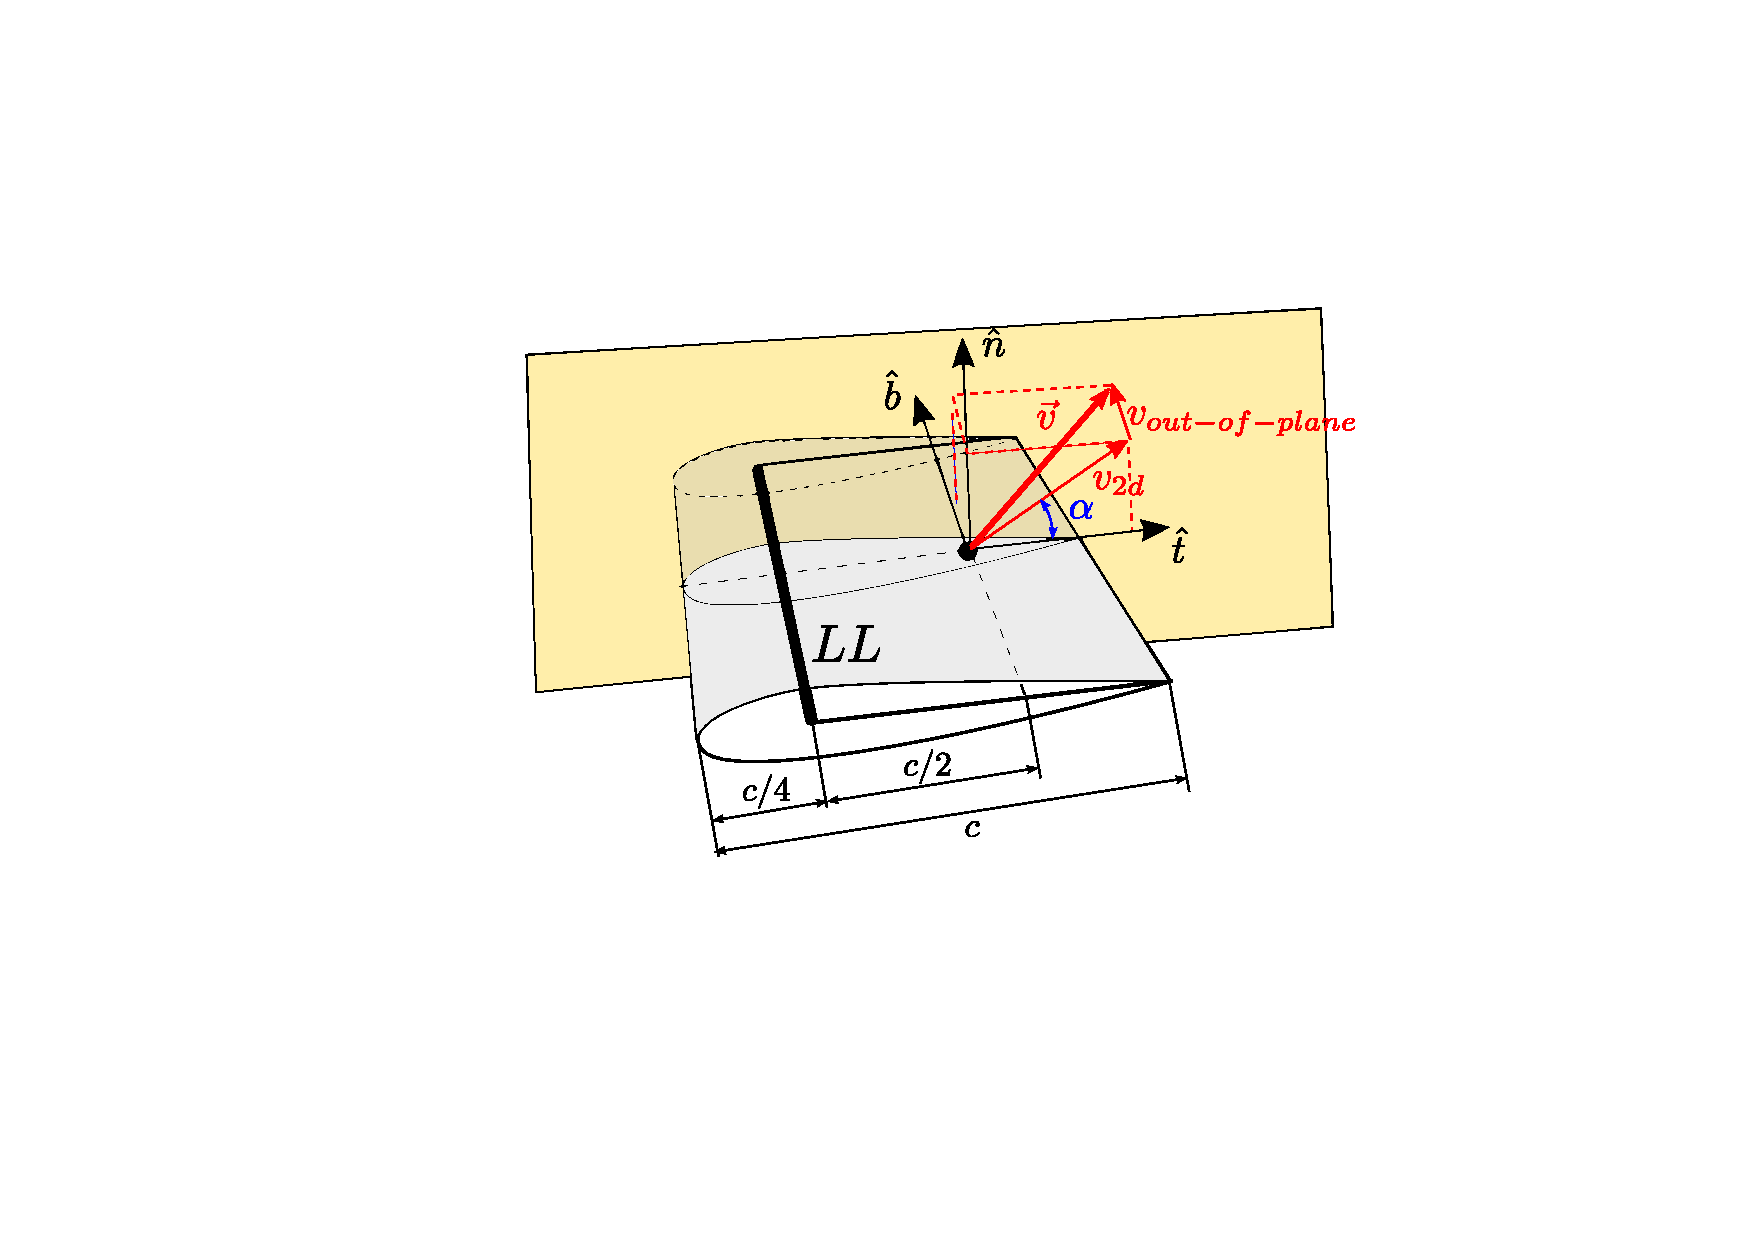
\includegraphics[width=1.0\textwidth, trim = 100 180 100 145, clip]{./images/ll_output_2} 
\caption{Lifting line data.}
\label{fig:ll_output}
\end{figure}



\subsection{Aeroacoustics}
The aeroacoustics postprocessing is a specific analysis used to 
extract from results all the various data required to perform an 
aeroacoustics analysis (with an external software) on the analysed results. 
It is available only in .dat ascii format  and it is intended rather than 
to be directly plotted/visualized to act as input for another software.

\begin{inputfile}[frame=single, caption={dust\_post.in for aeroacoustics}, 
  label={file:dust_post.in_aeroacoustics}]
!--- Data Names ---
data_basename = ./Output/sim_results
basename =     ./Postpro/postpro_output

analysis = {

type = aeroacoustics
name = aer01
start_res = 1
end_res   = 100 
step_res  = 1
format = dat

component = wing
component = tail

}
\end{inputfile}

\begin{itemize}
\item \param{type}: \textit{required:} one for each \param{analysis}. \textit{multiple:} no

type of the analysis, \opt{aeroacoustics} for aeroacoustics data

\item \param{name}: \textit{required:} one for each \param{analysis}. \textit{multiple:} no

name of the analysis, will be appended as a suffix to \param{basename}

\item \param{start_res}: \textit{required:} one for each \param{analysis}. 
\textit{multiple:} no

First result in the time series of the solver results to analyse.

\item \param{end_res}: \textit{required:} one for each \param{analysis}. 
\textit{multiple:} no

Last result in the time series of the solver results to analyse.

\item \param{step_res}: \textit{required:} one for each \param{analysis}. 
\textit{multiple:} no

Stride to employ when loading the time series of the solver results. 

\item \param{format}: \textit{required:} one for each \param{analysis}. 
\textit{multiple:} no

format of the processed results, can only be \opt{dat} for formatted ascii 
files output in case of aeroacoustics data analysis

\item \param{component}: \textit{required:} no. \textit{multiple:} yes. 
\textit{default:} all components.

Components to include in the aeroacoustics data. Only the data of the 
selected components will be included in the output file. 

\end{itemize}
